\section{Falsification commitments}
\label{sec:falsification}

This section is set apart as a separate structural level, rather than as a paragraph inside the Discussion, for a reason we state openly. \DEIC{} claims a scope that in academic psychology traditionally draws scepticism --- not because scope itself is suspect, but because broad frameworks have historically rarely said \emph{at what observation they would recognize themselves as wrong}. We draw this boundary ourselves, up front and in plain sight. Below is a list of predictions, each formulated together with its falsifier: the observation at which the prediction should be considered refuted. Refuting any of them individually means a local update of the framework; refuting the particular combinations specified in §\ref{subsec:collapse_thresholds} means that \DEIC{} as a scaffolding requires structural revision or retraction.

Formally, this is not a promise to be right. It is a commitment to recognize when we are wrong, and a commitment --- as to exactly which places and on exactly which data the test will be carried out.

\subsection{Orientation in the commitments table}
\label{subsec:falsification_guide}

Each commitment below has four components: \textbf{(1)}~the claim (what \DEIC{} predicts or posits), \textbf{(2)}~the falsifier (what observation makes the claim false), \textbf{(3)}~test requirements (what design, what sample size, what instrumental configuration are needed for the test to have force), \textbf{(4)}~consequence of refutation (what exactly in the framework is revised, rather than merely weakened). The commitments are grouped into five tiers: measurement (Tier~A), causal-path (Tier~B), topological (Tier~C), architectural (Tier~D) and programmatic (Tier~E).

\begin{figure}[htbp]
\centering
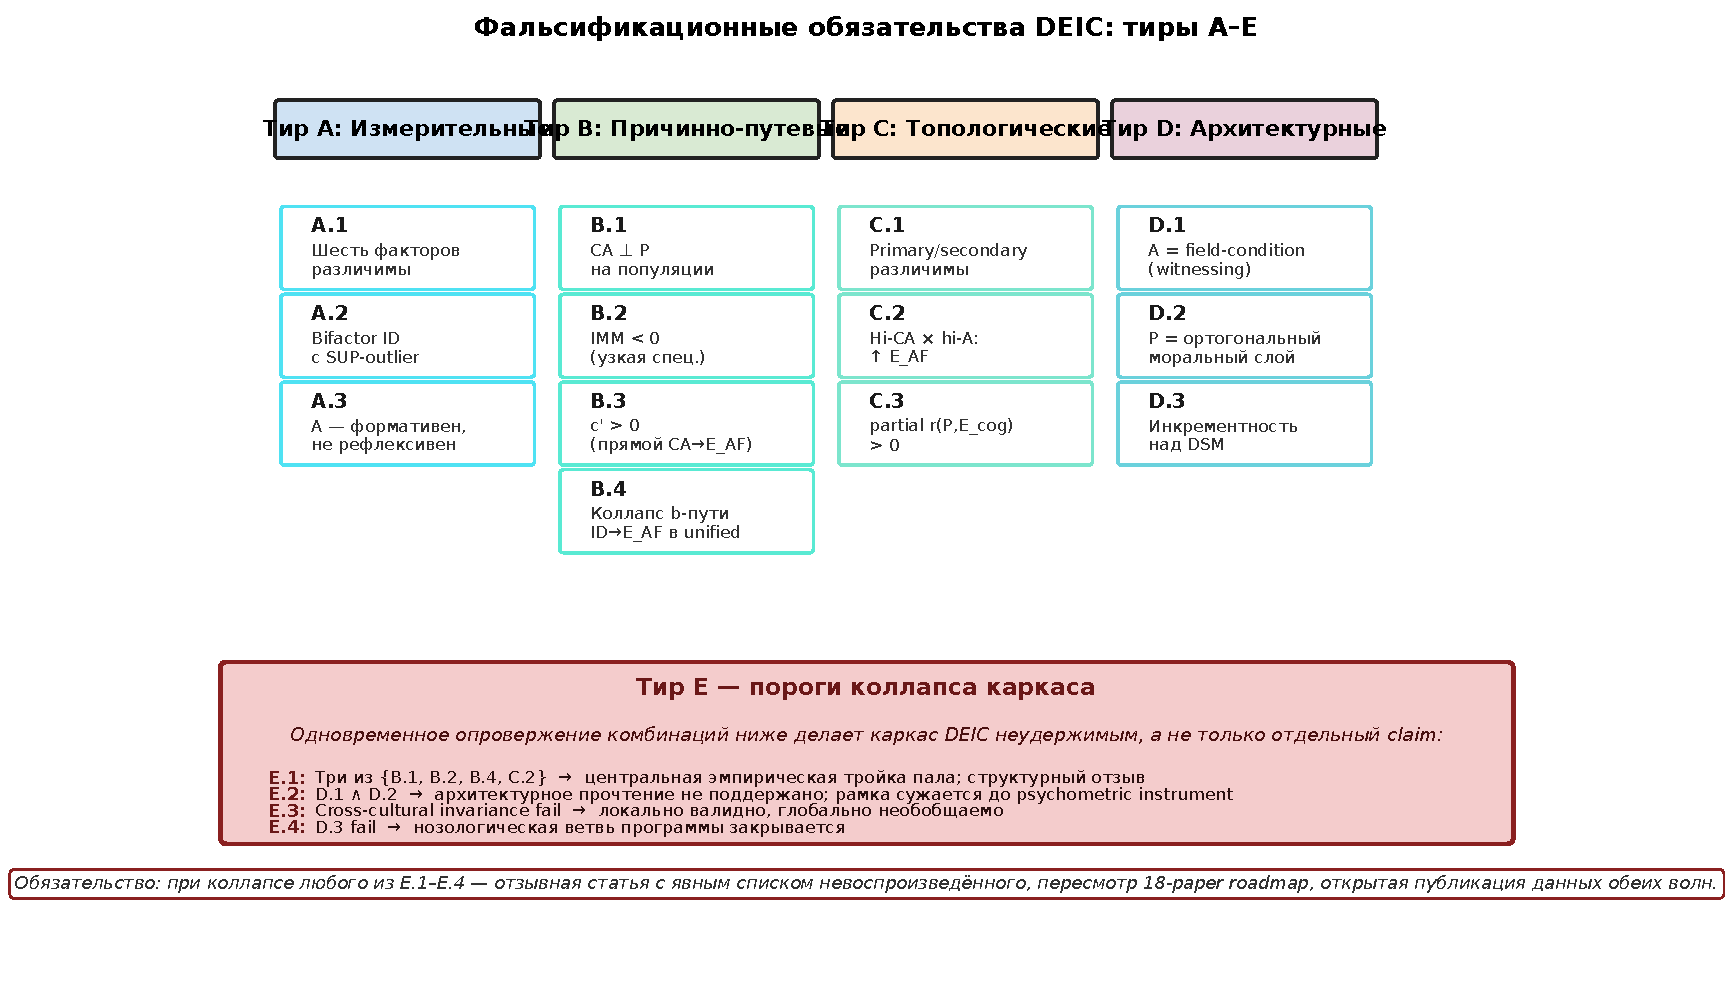
\includegraphics[width=0.95\linewidth]{figures/fig10_falsification_map.pdf}
\caption[Map of falsification commitments]{Map of \DEIC{}'s falsification commitments. Four tiers of local tests (A --- measurement; B --- causal paths; C --- topology; D --- architecture) form the upper row, each with its own commitments. The lower red band --- Tier~E: programmatic collapse thresholds at which the scaffolding is subject to structural revision rather than local update.}
\label{fig:falsification_map}
\end{figure}

The formulations are deliberately binary. Science does not work in binary modes --- but commitments do: either we are prepared to recognize a result as refutation, or we rule it out of the test ahead of time, in which case it is not a commitment.

\subsection{Tier A: measurement commitments}
\label{subsec:falsification_tier_a}

\paragraph{A.1 --- Six factors are distinguishable.}
\emph{Claim.} The six-factor oblique CFA (ID, CA, P, M, \EAF{}, \Ecog{}) is robustly reproduced on pre-registered items designed to separate the constructs.
\emph{Falsifier.} In wave~2, with items separated by design ($N \geq 1000$), either \EAF{} and \Ecog{} merge into a single empathy factor (CFI of the model with combined E is no worse than with separated by $\Delta$CFI $\leq 0.01$), or ID and CA are indistinguishable as separate latents ($r_{\mathrm{lat}} > 0.90$), or P and M are indistinguishable under instrumental independence.
\emph{Test requirements.} Pre-registered design; items for \EAF{} and \Ecog{} written on different content-specific constructs, not sharing common words. $N \geq 1000$ for stable CFA on 6 factors.
\emph{Consequence of refutation.} The multidimensional architecture of empathy in its current form is not supported; \DEIC{} narrows to the factor structure the data sustain (possibly four- or five-factor).

\paragraph{A.2 --- Bifactor structure of ID with SUP as separate.}
\emph{Claim.} The ID umbrella is better described by a bifactor model (general ID$_{\mathrm{g}}$ plus five uncorrelated specific factors) than by a unidimensional one, under $\Delta\chi^2$ at $p < 0.001$. Per-subscale ECV for SUP remains below $0.45$, for FLA above $0.70$.
\emph{Falsifier.} In wave~2 the bifactor model does not exceed the unidimensional one under $\Delta\chi^2$ at $p < 0.01$, OR ECV for SUP $> 0.55$ (SUP is equally well absorbed by general ID), OR ECV for FLA $< 0.45$ (FLA ceases to be a pure indicator of general ID).
\emph{Test requirements.} $N \geq 1200$ with items for SUP reconstructed as a standalone latent by design in wave~2.
\emph{Consequence of refutation.} The hypothesis that ``passive blocking is a single architecture with surface variations'' is revised; re-segmentation of ID into two independent latents is possible.

\paragraph{A.3 --- A is formative, not reflective.}
\emph{Claim.} A in the current instrument works as a formative composite. A dedicated A-scale, designed to isolate witnessing (observation-of-observation without trauma hypervigilance), will yield a reflective unifactorial CFI $\geq 0.93$ and reproduce a negative \IMM{} in the narrow specification.
\emph{Falsifier.} A dedicated witnessing-A-scale yields a single-latent CFI $\geq 0.95$ \emph{and} an \IMM{} that reproduces the sign and direction of the composite $-0.00197$ (CI does not include zero) --- then A is reflective, and our argument for its formativity is false. Or, conversely, the witnessing scale yields CFI $< 0.85$ and non-significant \IMM{} --- then neither operationalization of A supports the witnessing-moderation hypothesis.
\emph{Test requirements.} Item-level separation of witnessing (Josipovic/Dunne/Grabovac-anchor items) and hypervigilance (trauma-focused items); $N \geq 800$; nested conditional-process SEM.
\emph{Consequence of refutation (either branch).} Either A is reinterpreted as a reflective construct (simplification), or the witnessing-moderation hypothesis is not supported (revision of the central claim about the role of attention).

\subsection{Tier B: causal-path commitments}
\label{subsec:falsification_tier_b}

\paragraph{B.1 --- CA$\perp$P at the population level.}
\emph{Claim.} In the parallel mediation CA$\to$\{ID, P, M\}$\to$\EAF{}, the CA$\to$P path remains close to zero ($|\beta| < 0.10$) in a replication with a sample comparable in CA-spectrum breadth.
\emph{Falsifier.} CA$\to$P $\beta > 0.20$ at $p < 0.01$ in a replication sample $N \geq 1000$ with a CA-instrument and P-instrument of comparable content.
\emph{Test requirements.} Replication on an independent sample; the CA-instrument covers the same spectrum (early relational neglect, abuse, emotional deprivation); the P-instrument preserves the proportion of moral and architectural signature.
\emph{Consequence of refutation.} Architectural orthogonality of P and CA is not supported; primary and secondary psychopathy become a continuum rather than topologically separate cells. Clinical consequence: the psychopathic pattern is reinterpreted as a (co-)outcome of childhood trauma, not a separate architecture.

\paragraph{B.2 --- \IMM{} in the narrow specification is negative.}
\emph{Claim.} In the conditional-process SEM without P in the $b$-equation, the \IMM{} of the CA$\to$ID$\to$\EAF{} channel is negative, with 95\% CI not including zero.
\emph{Falsifier.} $P(\mathrm{IMM} < 0) < 0.90$ under any of the three reference Bayesian priors on a replication sample, OR the CI of the frequentist estimate crosses zero at $N \geq 1000$ with comparable A-composite structure.
\emph{Test requirements.} A-composite with comparable weighting structure; replication conducts parallel Bayesian and frequentist analyses.
\emph{Consequence of refutation.} The central result of the paper (two-stage A-moderation of CA$\to$ID$\to$\EAF) is not supported; A as moderator of the channel in the narrow specification is revised.

\paragraph{B.3 --- $c'$ (direct path CA$\to$\EAF{}) is positive.}
\emph{Claim.} After partialling ID, P, M and A, the direct path CA$\to$\EAF{} remains positive ($+0.15$--$+0.25$) --- ``raw'' childhood trauma does not kill empathy by itself; the defensive cascade kills it.
\emph{Falsifier.} $c' < -0.10$ with $p < 0.01$ in a replication, after correct partialling.
\emph{Test requirements.} Replication preserving the mediator structure; control for response bias (Lie as a covariate of \EAF).
\emph{Consequence of refutation.} The key thesis of the introduction (``trauma is not a verdict; defense transmits it'') loses its empirical footing; the \DEIC{} framework shifts to the more standard ``trauma $\to$ emotional damage'' narrative.

\paragraph{B.4 --- In the unified SEM the $b$-path ID$\to$\EAF{} collapses.}
\emph{Claim.} With all paths estimated simultaneously in the unified SEM the ID$\to$\EAF{} coefficient drops to statistical non-significance ($|\beta| < 0.10$, $p > 0.05$), and P$\to$\EAF{} dominates.
\emph{Falsifier.} In replication, the $b$-path ID$\to$\EAF{} remains $\beta < -0.20$ at $p < 0.001$ even with P included in the same equation.
\emph{Test requirements.} Replication of the unified SEM with the same latent structure.
\emph{Consequence of refutation.} The separation of ``architectural'' and ``narrative'' layers in the $E_{\mathrm{AF}}$ model is not supported; P and ID turn out to be additive rather than hierarchical mediators, and the theoretical separation of orthogonal channels requires revision.

\subsection{Tier C: topological commitments}
\label{subsec:falsification_tier_c}

\paragraph{C.1 --- Primary and secondary psychopathy are topologically distinguishable.}
\emph{Claim.} In the hi-P subsample ($N \geq 200$) bimodality is observed along the ID axis (or, in a multidimensional version, two distinct clusters in the ID$\times$CA plane), corresponding to the Karpman distinction: a primary cell (ID $\approx 0$, CA $\approx 0$) and a secondary cell (ID $> +0.5$, CA $> +0.5$).
\emph{Falsifier.} In the hi-P subsample $N \geq 200$ the Hartigan dip test gives no evidence of bimodality ($p > 0.1$), OR a Gaussian mixture on (ID, CA, A) gives a better BIC for $k=1$ than for $k=2$.
\emph{Test requirements.} Replication on an independent sample; preferably clinically enriched with a hi-P subgroup.
\emph{Consequence of refutation.} The Karpman distinction on \DEIC{}-coordinates is not supported; the topological $2\times2$ collapses into continuum psychopathy, as in much of contemporary literature. Clinical consequence: different interventions for ``primary'' and ``secondary'' types lose their footing.

\paragraph{C.2 --- The integrated survivor has elevated \EAF{}.}
\emph{Claim.} The hi-CA $\times$ hi-A cell ($\geq$ medians on each axis; expected share $\sim 15$--$18\%$ of the sample) has \EAF{} exceeding the median of the overall sample and exceeding the hi-CA $\times$ lo-A cell by at least $0.4\sigma$.
\emph{Falsifier.} $\mathrm{mean}\ \mathrm{E_{AF}}$ in the hi-CA $\times$ hi-A cell is at or below the overall sample median ($\Delta \leq 0$), OR the difference from hi-CA $\times$ lo-A $< 0.2\sigma$ in a replication $N \geq 1000$.
\emph{Test requirements.} Replication with analogous operationalization of A (composite or an equivalent witnessing scale); sample includes sufficient hi-CA representation ($\geq 25\%$).
\emph{Consequence of refutation.} The central publicly-significant claim that witnessing work compensates for the CA effect on affective empathy is not supported; ``trauma is not a verdict'' as an empirical claim is withdrawn and remains as a clinical horizon without statistical footing.

\paragraph{C.3 --- Partial $r$(P, \Ecog) is positive.}
\emph{Claim.} After partialling ID and CA, the partial correlation of P and \Ecog{} remains positive ($> +0.15$). This is explained by hyper-instrumentation: the P-pattern uses recognition of others' states selectively and is not deficient on the cognitive-E axis.
\emph{Falsifier.} Partial $r$(P, \Ecog{} \textbar{} ID, CA) $\leq 0$ in a replication $N \geq 1000$ with comparable separation of \EAF{}/\Ecog{}.
\emph{Test requirements.} The \Ecog{} scale is written on perspective-taking and understanding-of-others, not on empathic concern; the P-scale preserves the moral and architectural proportions; items do not share words.
\emph{Consequence of refutation.} The hyper-instrumentation hypothesis of Blair/Baron-Cohen is not reproduced in our data; the ``classical'' description of psychopathy as deficient on both forms of empathy turns out to be more accurate. The framing ``architecture, not deficit'' on the E axis weakens.

\subsection{Tier D: architectural commitments}
\label{subsec:falsification_tier_d}

\paragraph{D.1 --- A as field-condition, not as content of the field.}
\emph{Claim.} A dedicated witnessing-A-scale, separated by design from trauma hypervigilance, gives the same sign and direction of channel moderation CA$\to$ID$\to$\EAF{} as the current A-composite. If, however, a pure hypervigilance scale is constructed (attention-to-the-internal only, without witnessing), it moderates the channel in the opposite direction or does not moderate it at all.
\emph{Falsifier.} Both scales (witnessing-only and hypervigilance-only) moderate the channel in the same direction in a replication, OR the witnessing scale does not moderate at all.
\emph{Test requirements.} Two parallel item sets, content-validated by experts in contemplative tradition and trauma psychology; the same SEM structure for both.
\emph{Consequence of refutation.} The ontological distinction witnessing vs content at the attention axis is not supported; A returns to the general ranks of components of dispositional attention; the connection to the non-dual contemplative tradition loses empirical footing (it remains theoretical).

\paragraph{D.2 --- P as orthogonal moral layer.}
\emph{Claim.} Cognitively-morally phrased P-items (``I believe that in my case such behavior is permissible'') yield $\beta$ on \EAF{} and partial correlations with architectural-P-items such that the P-composite preserves $\approx$ half its variance as a moral component and $\approx$ half as architectural. P-moral alone remains orthogonal to CA ($|\beta| < 0.10$).
\emph{Falsifier.} After separating P into P-moral and P-arch in wave~2 both components either have $r_{\mathrm{lat}} > 0.85$ (indistinguishable), or P-moral correlates with CA at $\beta > +0.25$.
\emph{Test requirements.} Pre-registered item split; $N \geq 1000$; explicit cognitively-moral vs architectural phrasings.
\emph{Consequence of refutation.} The moral layer of P is not distinguishable from the architectural one; the interpretation of psychopathy as ``conditional coupling plus narrative of permission'' becomes internally inoperable and reduces to a single architectural component. The ethical framing ``architecture is morally neutral; narrative is evaluable'' loses its empirical cut-off.

\paragraph{D.3 --- Incremental validity of the \DEIC{} profile over the DSM label.}
\emph{Claim.} In retrospective re-analysis of clinical datasets with treatment response as outcome, the baseline \DEIC{} profile explains at least 5\% of additional variance in response after partialling out the DSM label.
\emph{Falsifier.} In retrospective on clinical data $N \geq 2000$ with measured \DEIC{} profile, incremental $R^2$ over DSM $< 0.05$.
\emph{Test requirements.} One or more clinical samples with parallel \DEIC{} measurement and DSM diagnosis; outcome: treatment response on a standardized metric (HAMD, PHQ, BDI, etc.).
\emph{Consequence of refutation.} The nosological claim of \DEIC{} as a trans-diagnostic stratifier is not supported; the framework narrows to a descriptive-theoretical role without a claim to clinical reorganization.

\paragraph{D.4 --- DI as an architectural marker, not an indicator of social desirability.}
\emph{Claim.} The magnitude of the declarative--behavioral gap $DI_{overall}$ tracks the defensive latent ID ($r \geq +0.30$) and the witnessing latent A ($r \leq -0.30$), and does not track clinical diagnosis ($|r| < 0.15$) in wave 2 on an independent sample. The prosocial-aligned version $DI_{aligned}$ remains structurally distinct from $piz$ ($|r| < 0.50$ with a sign opposite to the one expected were DI a self-presentation indicator).
\emph{Falsifier.} In wave 2 ($N \geq 800$), either $|r(DI_{overall}, \text{ID})| < 0.30$, or $|r(DI_{overall}, \text{dx\_any})| > 0.20$, or $r(\text{piz}, DI_{aligned}) > +0.30$ (turning DI into a sub-component of $piz$ without an independent disposition).
\emph{Test requirements.} Wave-2 inventory preserving the principle of paired declarative/behavioral formulations on all scales of the ID perimeter; re-measurement of dx and $piz$ on the same sample; re-fit of the 6-factor oblique CFA with latent scores.
\emph{Consequence of refutation.} DI as an independent architectural metric is not supported: either the gap does not track architecture, or it tracks the clinical profile (which moves DI into a diagnostic rather than architectural category), or it is fully explained by $piz$ (a pure SD artifact). In any of these cases, §\ref{subsec:di_asymmetry} and the interpretation of DI in §\ref{subsec:di_results} require retraction; \texttt{extended\_metrics.DI} in the instrument moves from an architectural marker to either a clinical one or a duplicate of $piz$, and its place in the wave-2 dashboard is reconsidered.

\subsection{Tier E: programmatic collapse thresholds}
\label{subsec:collapse_thresholds}

Up to this point each commitment has been described as a local test with a local consequence. But \DEIC{} is not a set of independent hypotheses --- it is an architecture with interdependent nodes. Refutation of certain combinations means that the scaffolding as a whole does not hold, and not merely that one branch has grown stale. We formulate these combinations explicitly.

\paragraph{E.1 --- Collapse of the central empirical triad.}
If three of the four central commitments are simultaneously refuted --- B.1 (CA$\perp$P), B.2 (\IMM{} negative), B.4 (collapse of $b$-path in unified), C.2 (integrated survivor with elevated \EAF) --- three of the empirical pillars on which the central argument of the paper is built are not reproduced. In that case \DEIC{} as an empirical framework requires \emph{structural revision, not update}: instrument version~2 and the accompanying theoretical framework must be retracted and replaced by a narrower working hypothesis with explicit indication of those fragments that at this point remain supported.

\paragraph{E.2 --- Collapse of the architectural reading.}
If D.1 (witnessing-moderation) and D.2 (distinguishability of P-moral and P-arch) are simultaneously refuted, the theoretical framework ``psychopathy as conditional coupling plus moral narrative; attention as field-condition'' is not supported. \DEIC{} in that case \emph{narrows to an empirical coordinate system} without architectural or ontological theses: fit for use as a psychometric instrument, but not as a framework claiming dialogue with the contemplative tradition and with moral philosophy.

\paragraph{E.3 --- Collapse of generalizability.}
If cross-cultural validation on non-Russian-speaking samples (EN, ES, CH, AR) shows that the six-factor CFA does not reproduce scalar invariance, and the central B.2 and C.2 reproduce only in \emph{part} of the cultural contexts, \DEIC{} remains a \emph{locally valid, globally non-generalizable} instrument. This is not a collapse of the framework as such, but a withdrawal of the claim that the described architecture is a universal device of the psyche rather than an artefact of Russian-language/late-Soviet cultural formation. The applied papers of the program (political communication, evolutionary psychology) are in that case restricted to the corresponding cultural range.

\paragraph{E.4 --- Collapse of the nosological claim.}
If D.3 (incremental validity over DSM) is refuted, the nosological branch of the program (the paper on the \DEIC{} profile as trans-diagnostic stratifier, §\ref{sec:future}) is closed until new grounds emerge. The framework remains descriptively scientific, but without claim to reorganization of clinical categories.

\paragraph{What ``the scaffolding is subject to revision'' means.}
We acknowledge: public retraction or structural revision is not the same as silence. In the event of collapse of any of levels E.1--E.4 we commit to \textbf{(i)}~publish a retraction paper with an explicit list of what is not reproduced and with an explicit reformulation of what remains; \textbf{(ii)}~revise the 18-paper publication roadmap --- some of the planned papers will lose their grounds and be withdrawn; \textbf{(iii)}~publish the data of both waves openly, so that other groups can conduct independent re-analyses. This commitment has the same form as the commitments of open methodological culture after the replication crisis in social psychology of the 2010s: not ``if we are wrong, we will rewrite history'', but ``if we are wrong, we will acknowledge it and release the data''.

\subsection{What this section means for reading the paper}
\label{subsec:falsification_closing}

We draw two consequences for the reader.

First. No statement in this paper should be read as a ``closed'' or ``proven'' fact. Each is a hypothesis with its own falsification boundary, formulated here. In the body of the paper --- in Results, in Discussion --- these statements are formulated in the findings register (``the data show'', ``the model yields''), as psychometric reporting requires. But the scientific status of each is determined not by that register, but by the presence of a formulated falsifier in this section.

Second. We do not regard falsification as a threat to the program. Refutation of a local prediction (any of A.1--D.3) is a normal course of empirical inquiry and a basis for an update. Refutation of a combination (E.1--E.4) is a normal course of scientific self-correction, and the program foresees this outcome as a possibility. The only outcome unacceptable to us is not refutation, but evasion: if statements are formulated such that they cannot be either confirmed or refuted, the work falls outside the boundaries of science regardless of its technical sophistication. The falsification section exists precisely to prevent such evasion. This --- a contribution we consider independent of whether the framework itself turns out to be valid.

In §\ref{sec:future} we formulate the concrete designs that will carry out each of the tests. In the open documentation of the program (\texttt{PROGRAM\_STRUCTURE.md}) the planned papers are listed with their mapping to Tiers A--E of this section.
